%
% File: introduction.tex
% Author: Victor F. Brena-Medina
% Description: Introduction chapter where the biology goes.
%
\let\textcircled=\pgftextcircled
\chapter{Introduction}

\initial{T}his chapter will be used to acquaint the reader with the emerging UAV market, and the challenges it is facing on its way towards maturity.
Also, the reasons for its rapid evolution will be exposed and finally, focusing on the contents of this thesis, the personal motivation and the methodology will be explained to further expand on the topics of interest in the following chapters.

\section{Background information} \label{sec:background}

The first remotely radio controlled models appeared in the early twentieth century as small prototypes for potential manned aircraft. 
Afterwards, and during most of the century, the investigation and development lines were directed towards the military scope, in which the main objective of UAVs, which is still applied today, was to substitute manned aircraft in three types of military operations, commonly known as ``the three D's" \cite{daily2015,uasapplications2016}:

\begin{itemize}
	\item Dirty: operations performed in a contaminated environment.
	\item Dangerous: operations entailing some risk for the pilot.
	\item Dull: long and monotone operations, such as monitoring operations.
\end{itemize}

In the 70's and the 80's, efforts were directed to improve the technical characteristics of these vehicles.
But it was not until the late 80's when a revolution in the industry took place with the introduction of the GPS navigation system, whose accuracy in geolocation opened a whole new spectrum of possibilities.

Regarding the civil sector, the potential applications of UAVs in the non-military field are much more diverse.
Nowadays these vehicles are in the process of finding new niche positions in the civilian market, having been introduced up to now in different industry sectors such as agriculture, forest fire fighting, search and rescue, aerial photography, cartography, or security and surveillance, among others. 
Despite the latter, the use of UAVs for civil purposes is relatively recent in comparison with the military sector.
This late implementation in the civilian field was caused mainly by two limitations which are of minor relevance in the fighting industry: legislation and economy.
\cite{aguado2016}

\section{Socioeconomic environment}

Apart from ``the three D's'' mentioned in Section \ref{sec:background}, another reason for the embracement of UAVs within the industry shall be considered.
The final goal of any company is to create profit to their shareholders, which can be done either by increasing the revenues or by decreasing the costs of their activities.
UAVs enter in the latter category.
The consistent usage of smaller tools as compared with the manned workpower usually means that the equipment costs can be lowered, as well as the man-hours needed to perform the task \cite{airbusdemonstratesaircraftinspectionbydroneatfarnborough2016}, not to mention that most of the time the number of workers needed can be reduced to as low as one or two, in charge of operating the UAS (Unmanned Aerial System\footnote{UAS refers to the bigger system that incorporates one or more UAVs, as well as the Ground Control Station or other related subsystems}).

This phenomenon is already proving to be very effective for the companies taking advantage of it, but research also shows an even bigger potential that is still waiting to be exploited, claiming that UAVs could have replaced \$127 billion worth of human labour in 2015 \cite{wisniewski2016}, distributed in the sectors shown in Figure \ref{fig:pwc}.

\begin{figure}[htb]
	\centering
	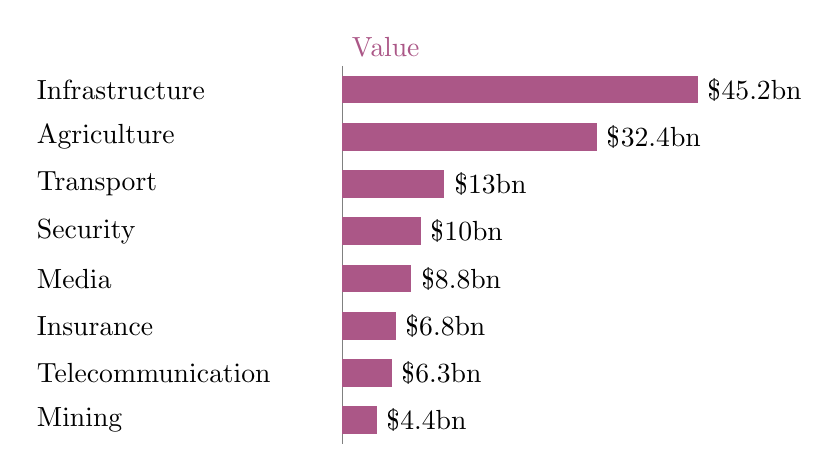
\begin{tikzpicture}

		\definecolor{purpleAtlas}{RGB}{171,87,135}

		%\draw[step=1cm,gray,very thin] (0,0) grid (10,6);

		\node[above right,purpleAtlas] at (4,6.1) {Value};
		\draw[black!50] (4,6.1) -- (4,1.3);
		\draw[purpleAtlas, line width=0.35cm] (4,5.8) -- (8.52,5.8);
			\node[right] at (0,5.8) {Infrastructure};
			\node[right] at (8.52,5.8) {\$45.2bn};
		\draw[purpleAtlas, line width=0.35cm] (4,5.2) -- (7.24,5.2);
			\node[right] at (0,5.2) {Agriculture};
			\node[right] at (7.24,5.2) {\$32.4bn};
		\draw[purpleAtlas, line width=0.35cm] (4,4.6) -- (5.3,4.6);
			\node[right] at (0,4.6) {Transport};
			\node[right] at (5.3,4.6) {\$13bn};
		\draw[purpleAtlas, line width=0.35cm] (4,4) -- (5,4);
			\node[right] at (0,4) {Security};
			\node[right] at (5,4) {\$10bn};
		\draw[purpleAtlas, line width=0.35cm] (4,3.4) -- (4.88,3.4);
			\node[right] at (0,3.4) {Media};
			\node[right] at (4.88,3.4) {\$8.8bn};
		\draw[purpleAtlas, line width=0.35cm] (4,2.8) -- (4.68,2.8);
			\node[right] at (0,2.8) {Insurance};
			\node[right] at (4.68,2.8) {\$6.8bn};
		\draw[purpleAtlas, line width=0.35cm] (4,2.2) -- (4.63,2.2);
			\node[right] at (0,2.2) {Telecommunication};
			\node[right] at (4.63,2.2) {\$6.3bn};
		\draw[purpleAtlas, line width=0.35cm] (4,1.6) -- (4.44,1.6);
			\node[right] at (0,1.6) {Mining};
			\node[right] at (4.44,1.6) {\$4.4bn};

	\end{tikzpicture}
	\caption{Distribution of potential UAV markets \cite{wisniewski2016}}
	\label{fig:pwc}
\end{figure}


\section{Legal framework}

Due to the fast-evolving UAV industry, the aviation authorities have not yet been able to develop a reasonable set of regulations and standards to harmonize the legislation across borders.
Aditionally, this regulatory framework should consider the idea that each system has unique capabilities and characteristics and also that development and innovation are very important concept in the field, and should not be dampened by restrictive rules \cite{valavanis2015}

However, there have already been some efforts from ICAO to outline some general rules to give a global sense of what is expected from the UAV sector \cite{manualonremotelypilotedaircraftsystemsrpas2015}. 
In addition to that, some countries are creating their own legislation to enable the operation of Unmanned Aerial Vehicles within their territory.

For example, the Spanish government issued an urgent provisional regulation on October 2014 \cite{ley182014de15deoctubredeaprobaciondemedidasurgentesparaelcrecimientolacompetitividadylaeficiencia2014} that affects to Remotely Piloted Aircraft Systems (RPAS\footnote{RPAS are considered as a subset of the UAS group. Fully automatic vehicles do not belong to the RPAS category, since the existance of a remote pilot is required at any time}) not exceeding 150 kg of Maximum Take Off Mass (MTOM). Heavier UAVs are subjected to European regulations \cite{regulationecno21620082008}
Focusing on the smaller segments, UAVs are separated according to their MTOM as follows:
\begin{description}
	\item[MTOM < 2 kg:] Flights Beyond Visual Line Of Sight (BVLOS) are allowed, but conditioned to the publication of a NOTAM (NOtice To AirMen). Apart from that, all the other rules in the 2 kg to 25 kg apply.
	\item[2 kg $\leq$ MTOM < 25 kg:] Only operable in areas separated from groups of buildings in cities, or groups of people elsewhere. Flight shall always take place in uncontrolled airspace, within Visual Line Of Sight (VLOS) and at a maximum distance of 500 m from the position of the pilot, not exceeding 400 ft of heigt over the terrain.
	\item[25 kg < MTOM:] Flight is only allowed for firefighting, search and rescue missions. They shall only operate in uncontrolled airspace and according to the limitations stablished in their Airworthiness Certificate, as emited by AESA.
\end{description}
Nevertheless, even if Spain or other countries have their own regulations to control the usage of UAVs in their territories, it is still important to have an international and stable legislation to allow the sector to grow to its full potential.


\section{Motivation}\label{sec:motivation}

Traditionally, the most important payload that could be carried in an aircraft was human beings, that would perform their mission while aloft.
Nevertheless, the advancements on sensing technology and wireless communications have forced a change on traditional aviation.
Apart from commercial aviation, where the final objective is to transport people form one place to another, in almost any other mission the role of the human workforce is to pilot the aircraft and/or operate the payload systems.
This secondary role of the human operators implies that, given the maturity of the involved technology, they could be substituted by intelligent computer systems or, at least, disembarked form the aircraft into a safer Ground Control Station (GCS).
The process of ``unmanning'' the aircraft also brings the advantages of decreasing the weight of the aircraft and thus improving its endurance and manoeuvrability, avoids putting the pilot in a dangerous situation, and helps alleviate the errors associated with tedious and repetitive tasks, among others.

However, there are also some downsides.
In the technical department, there are still some issues regarding the electromagnetic spectrum allocation for the data-link with the vehicle \cite{civilianunmannedaerialvehiclesreadyfortakeoff2012}, as well as accommodating unmanned aircraft within the Airspace System \cite{unmannedaircraftsystemsperceptionsandpotentials2013}.
In addition, the most accused issues for experienced pilots are those related with the loss of situational awareness that comes as a result of eliminating the physical cues (body inertia, vibrations\ldots) and relying on instrumental readings only \cite{bergqvist2014}.
Hence, some enhanced systems need to be integrated into the vehicle to overcome this limitations, providing the pilots with additional information for the safe execution of the mission.

Finally, for this project, the goal is to provide a system that reduces the possibility of it crashing with nearby obstacles, so that regular operations are carried with a higher level of safety.
Eventually, the authorities could consider the increase in overall safety as a standard, triggering the modification of existing regulations to a more permissive set, and allowing the industry to take advantage of all the benefits that the incorporation of UAVs could bring to their activities.

\section{Project objectives} \label{sec:objectives}

According to the motivation as stated in Section \ref{sec:motivation}, the final goal of this project is to develop a working prototype for proof of concept of a system able to detect and avoid obstacles that threaten the integrity of the UAV. Towards that end, some more specific objectives can be defined as follows:
\begin{itemize}
	\item Identify the requirements needed for the Obstacle Collision Avoidance System (OCAS) to correctly fulfill its purpose
	\item Define the functional architecture of the OCAS
	\item Define the interfaces (communication channels and protocols) to be used by the OCAS for its correct integration on the UAV
	\item Define the interaction channels and procedures between the UAV equiped with OCAS and Ardupilot and the operator
	\item Develop a first working prototype as proof of concept of the Obstacle Collision Avoidance System (both hardware and software) and integrate it on a real UAV
\end{itemize}

\section{Methodology}

As some may have noticed, the objectives defined in Section \ref{sec:objectives} remember of the first steps that are usually taken in the Systems Engineering approach for interdisciplinary design \cite{whatissystemsengineering}.
That approach will be adapted to the project, and some useful tools and concepts will be used \cite{nationalaeronauticsandspaceadministration2007}, such as the requirements capture, the Functional Flow Block Diagram (FFBD), the Functional Architecture definition or the product integration via interfaces definition.

Finally the prototype created from the process will be tested in a series of common situations to prove that the product is capable of completing its task.
Also, it will be demonstrated how the OCAS has been designed with flexibility and modularity in mind, explaining the possibilities to expand its features and proposing some ideas for future work.

\section{Time planning}

For any big project with defined deadlines, time management is of utmost importance.
The elaboration of the thesis has been carried out during more than 10 months, and the different work phases have been monitored with a project management software tool.
The resulting Gantt Diagram can be consulted on Figure \ref{fig:gantt}.

\begin{figure}[htbp!]
	\hspace{-3cm}
	%\centering
	\begin{ganttchart}[
		time slot format=little-endian,
		x unit=0.045cm,
		y unit chart=0.48cm,
		y unit title=0.7cm,
		group height=0.3,
		group peaks height=0.2,
		group peaks width=3,
		group peaks tip position=0,
		group/.append style={fill=teal!40},
		group label node/.append style={align=right},	% to enable line breaks
		group label font=\bfseries\small,
		bar height=0.7,
		bar/.append style={fill=teal!80,draw=none},
		bar label node/.append style={align=right},	% to enable line breaks
		bar label font=\small,
		milestone height=0.5,
		milestone right shift=2,
		milestone left shift=-2,
		milestone/.append style={fill=purpleAtlas,draw=none},
		title/.style={fill=teal!80!black},
		title label font=\color{white},
		newline shortcut=true,
		]
		{01-11-2015}{26-09-2016}

		\gantttitlecalendar{year,month} \ganttnewline

		\ganttbar{\bfseries Problem statement \\ \bfseries Objectives definition}{01-11-2015}{15-11-2015} \\ \\
		\ganttmilestone{Objectives defined}{15-11-2015} \\

		\ganttgroup[group/.append style={fill=teal}]{State of the Art}{01-11-2015}{05-05-2016}\\

			\ganttbar{Legislation study}{01-11-2015}{10-11-2015} \\

		\ganttgroup{Familiarisation with F450}{01-11-2015}{17-11-2015} \\
			\ganttbar{GCS software tools}{01-11-2015}{04-11-2015} \\
			\ganttbar{Data-link range improvement}{05-11-2015}{17-11-2015} \\ \\

		\ganttgroup{Familiarisation with \\ Arduino/Electronics}{18-11-2015}{29/02/2016} \\ \\
			\ganttbar{Default sensors}{18-11-2015}{10-12-2015} \\ 
			\ganttbar{Additional sensors}{11-12-2015}{18-12-2015} \\
			\ganttbar{Serial communication}{25-01-2016}{23-02-2016} \\ 
			\ganttbar{GPS study}{12-02-2016}{29-02-2016} \\ 

		\ganttgroup{Modular payload}{08-02-2016}{07-03-2016} \\
			\ganttbar{Ardupilot study}{08-02-2016}{11-02-2016} \\
			\ganttbar{Build new platform}{01-03-2016}{02-03-2016} \\
			\ganttbar{Calibration}{02-03-2016}{07-03-2016} \\

		\ganttgroup{SITL setup}{08-03-2016}{31-03-2016} \\
			\ganttbar{MAVproxy}{08-03-2016}{14-03-2016} \\
			\ganttbar{MAVproxy}{15-03-2016}{31-03-2016} \\

		\ganttgroup{No-fly Zrone}{01-04-2016}{05-05-2016} \\
			\ganttbar{Alternative position determination}{05-04-2016}{07-04-2016} \\
			\ganttbar{Electromagnetic radiation}{08-04-2016}{12-04-2016} \\
			\ganttbar{Stereoscopic cameras}{13-04-2016}{21-04-2016} \\
			\ganttbar{Stereoscopic tests}{25-04-2016}{05-05-2016} \\

		\ganttgroup[group/.append style={fill=teal}]{Problem solving}{01-06-2016}{31-07-2016} \\

			\ganttbar{Platform assembly}{01-06-2016}{03-06-2016} \\
			\ganttbar{Platform calibration}{03-06-2016}{06-06-2016} \\
			\ganttmilestone{Test platform ready}{06-06-2016} \\

			\ganttbar{Software coding on GCS}{06-06-2016}{17-06-2016} \\
			\ganttbar{Software testing on GCS}{17-06-2016}{28-06-2016} \\

			\ganttbar{Raspberry Pi deployment}{22-06-2016}{30-06-2016} \\

			\ganttbar{GUI deployment}{04-07-2016}{05-07-2016} \\

			\ganttbar{Sonar integration}{08-07-2016}{14-07-2016} \\
			\ganttbar{Dronekit scripts incorporation}{14-07-2016}{25-07-2016} \\
			\ganttbar{Final tests}{26-07-2016}{31-07-2016} \\

			\ganttmilestone{Software frozen}{31-07-2016} \\

		\ganttgroup[group/.append style={fill=teal}]{Memoir writting}{01-08-2016}{31-08-2016} \\

		\ganttmilestone{Thesis hand-in}{23-09-2016}

	\end{ganttchart}
	
	\caption{Gantt Diagram of the Project}
	\label{fig:gantt}
\end{figure}


It is worth mentioning that in the period from 01/11/2015 to 05/05/2016 I was doing my professional internships at Centum Solutions.
Thus, most of my research during that time was guided by the interests of the company.
Nevertheless, that stage proved very useful for the summer period, when my work was exclusively focused towards my thesis.

\section{Budget}



